%%%%%%%%%%%%%%%%%%%%%%%%%%%%%%%%%%%%%%%%%
% Structured General Purpose Assignment
% LaTeX Template
%
% This template has been downloaded from:
% http://www.latextemplates.com
%
% Original author:
% Ted Pavlic (http://www.tedpavlic.com)
%
% Note:
% The \lipsum[#] commands throughout this template generate dummy text
% to fill the template out. These commands should all be removed when
% writing assignment content.
%
%%%%%%%%%%%%%%%%%%%%%%%%%%%%%%%%%%%%%%%%%

%----------------------------------------------------------------------------------------
%	PACKAGES AND OTHER DOCUMENT CONFIGURATIONS
%----------------------------------------------------------------------------------------

\documentclass{article}

\usepackage{fancyhdr} % Required for custom headers
\usepackage{lastpage} % Required to determine the last page for the footer
\usepackage{extramarks} % Required for headers and footers
\usepackage{graphicx} % Required to insert images
\usepackage{lipsum} % Used for inserting dummy 'Lorem ipsum' text into the template
\usepackage{enumerate}
\usepackage{booktabs}
\usepackage{amsmath}

% Margins
\topmargin=-0.45in
\evensidemargin=0in
\oddsidemargin=0in
\textwidth=6.5in
\textheight=9.0in
\headsep=0.25in

\linespread{1.5} % Line spacing

% Set up the header and footer
\pagestyle{fancy}
\lhead{\hmwkAuthorName} % Top left header
\chead{\hmwkClass\ (\hmwkTitle)} % Top center header
%%\rhead{\firstxmark}
\rhead{} % Top right header
\lfoot{\lastxmark} % Bottom left footer
\cfoot{} % Bottom center footer
\rfoot{Page\ \thepage\ of\ \pageref{LastPage}} % Bottom right footer
\renewcommand\headrulewidth{0.4pt} % Size of the header rule
\renewcommand\footrulewidth{0.4pt} % Size of the footer rule

\setlength\parindent{0pt} % Removes all indentation from paragraphs

%----------------------------------------------------------------------------------------
%	DOCUMENT STRUCTURE COMMANDS
%	Skip this unless you know what you're doing
%----------------------------------------------------------------------------------------

% Header and footer for when a page split occurs within a problem environment
\newcommand{\enterProblemHeader}[1]{
\nobreak\extramarks{#1}{#1 continued on next page\ldots}\nobreak
\nobreak\extramarks{#1 (continued)}{#1 continued on next page\ldots}\nobreak
}

% Header and footer for when a page split occurs between problem environments
\newcommand{\exitProblemHeader}[1]{
\nobreak\extramarks{#1 (continued)}{#1 continued on next page\ldots}\nobreak
\nobreak\extramarks{#1}{}\nobreak
}

\setcounter{secnumdepth}{0} % Removes default section numbers
\newcounter{homeworkProblemCounter} % Creates a counter to keep track of the number of problems

\newcommand{\homeworkProblemName}{}
\newenvironment{homeworkProblem}[1][Problem \arabic{homeworkProblemCounter}]{ % Makes a new environment called homeworkProblem which takes 1 argument (custom name) but the default is "Problem #"
\stepcounter{homeworkProblemCounter} % Increase counter for number of problems
\renewcommand{\homeworkProblemName}{#1} % Assign \homeworkProblemName the name of the problem
\section{\homeworkProblemName} % Make a section in the document with the custom problem count
\enterProblemHeader{\homeworkProblemName} % Header and footer within the environment
}{
\exitProblemHeader{\homeworkProblemName} % Header and footer after the environment
}

\newcommand{\problemAnswer}[1]{ % Defines the problem answer command with the content as the only argument
\noindent\framebox[\columnwidth][c]{\begin{minipage}{0.98\columnwidth}#1\end{minipage}} % Makes the box around the problem answer and puts the content inside
}

\newcommand{\homeworkSectionName}{}
\newenvironment{homeworkSection}[1]{ % New environment for sections within homework problems, takes 1 argument - the name of the section
\renewcommand{\homeworkSectionName}{#1} % Assign \homeworkSectionName to the name of the section from the environment argument
\subsection{\homeworkSectionName} % Make a subsection with the custom name of the subsection
\enterProblemHeader{\homeworkProblemName\ [\homeworkSectionName]} % Header and footer within the environment
}{
\enterProblemHeader{\homeworkProblemName} % Header and footer after the environment
}

%----------------------------------------------------------------------------------------
%	NAME AND CLASS SECTION
%----------------------------------------------------------------------------------------

\newcommand{\hmwkTitle}{Homework\ \#7} % Assignment title
\newcommand{\hmwkDueDate}{Tuesday,\ April\ 10,\ 2018} % Due date
\newcommand{\hmwkClass}{FIN\ 513} % Course/class
\newcommand{\hmwkClassTime}{9:30am} % Class/lecture time
\newcommand{\hmwkAuthorName}{Wanbae Park} % Your name

%----------------------------------------------------------------------------------------
%	PARTIAL DERIVATIVES
%----------------------------------------------------------------------------------------
\newcommand{\pdv}[3][]{
	\frac{\partial^{#1}{#2}}{\partial{{#3}^{#1}}}
}

%----------------------------------------------------------------------------------------
%	EXPECTATION AND VARIANCE OPERATOR
%----------------------------------------------------------------------------------------
 \newcommand{\E}{\mathrm{E}}
 \newcommand{\Var}{\mathrm{Var}}
 \newcommand{\Cov}{\mathrm{Cov}}
 \newcommand{\Corr}{\mathrm{Corr}}

%----------------------------------------------------------------------------------------
%	TITLE PAGE
%----------------------------------------------------------------------------------------

\title{
\vspace{2in}
\textmd{\textbf{\hmwkClass:\ \hmwkTitle}}\\
\normalsize\vspace{0.1in}\small{Due\ on\ \hmwkDueDate}\\
\vspace{3in}
}

\author{\textbf{\hmwkAuthorName}}
\date{} % Insert date here if you want it to appear below your name

%----------------------------------------------------------------------------------------

\begin{document}


\maketitle

%----------------------------------------------------------------------------------------
%	TABLE OF CONTENTS
%----------------------------------------------------------------------------------------

%\setcounter{tocdepth}{1} % Uncomment this line if you don't want subsections listed in the ToC

%%\newpage
%%\tableofcontents
\newpage

%----------------------------------------------------------------------------------------
%	PROBLEM 1
%----------------------------------------------------------------------------------------

% To have just one problem per page, simply put a \clearpage after each problem

\begin{homeworkProblem}
	\begin{enumerate}[(a)]
		\item	%% problem (a)
		\textbf{Disagree.} Under CAPM, market price of risk for an arbitrary
		asset is defined as $\lambda_X = \rho_{X, M} \lambda_M$, where $X$
		is an arbitrary asset, and $M$ denotes market.
		Let $X$ denotes temperature, and if temperature increases are
		associated with lower stock prices, it means that correlation
		between temperature and stock price, $\rho_{X, M}$, is negative.
		Since market price of risk associated with stock price is positive,
		which associated with global warming will be negative, not positive.
		\item	%% problem (b)
		\textbf{Agree.}
		From the equation $\lambda_X = \rho_{X, M} \lambda_M$, market price
		of risk for an arbitrary asset is calculated as multiple of
		correlation coefficient between the asset and market
		and Sharpe ratio for the stock market.
		Since correlation coefficient is between -1 and 1, its absolute
		value must be smaller than the Sharpe ratio for the stock market.
	\end{enumerate}
\end{homeworkProblem}

%----------------------------------------------------------------------------------------
%	PROBLEM 2
%----------------------------------------------------------------------------------------

\begin{homeworkProblem}
	\begin{enumerate}[(a)]
		\item	%% problem (a)
		Since the market price of volatility risk is given as
		$\lambda(v) = \lambda_0 + \lambda_1 v$, risk-neutralized process
		of $v$ is derived as follows.
		%% EQUATION
		\begin{equation*}
			\begin{aligned}
				dv_t 	&= \kappa(\bar{v} - v_t)dt - \lambda(v) s_v dt + s_vdW_t^v	\\
						&= (\kappa \bar{v} - \lambda_0 s_v -
							(\kappa + \lambda_1 s_v)v_t)dt
							+ s_v dW_t^v	\\
						&= k^* (\bar{v}^* - v_t)dt + s_v dW_t^v	\\
			\end{aligned}
		\end{equation*}
		where $\kappa^* = \kappa + \lambda_1 s_v$, and
		$\bar{v}^* = \frac{\kappa \bar{v} - \lambda_0 s_v}{\kappa^*}$.
		Since $\kappa^*$ and $\bar{v}^*$ are constant, $v_t$ follows
		Ornstein-Uhlenbeck process under risk-neutral measure.
		\item	%% problem (b)
		Let $F$ denote forward price for the contract.
		If there is no arbitrage opportunity, $F$ should satisfy the following
		equation.
		\begin{equation*}
			\begin{aligned}
				\E^*[B_{0, T} (\sigma_T - F)] = 0	\\
				\Rightarrow F = \E^*[\sigma_T]
			\end{aligned}
		\end{equation*}
		Where $B_{0, T}$ denotes discount factor from current date to the
		maturity and $\E^*$ denotes expectation operator under risk-neutral
		measure.
		It is known that a random variable which follows Ornstein-Uhlenbeck
		process is normally distributed, so $v_t = \log \sigma_t^2$ is
		normally distributed. Therefore, there is a closed form of $\E^*[\sigma_T]$.
		From the analogy of distribution in lecture note 7.2, $v_T$ is distributed
		as $N(v_0 e^{-\kappa^* T} + \bar{v}^* (1 - e^{\kappa^* T}),
			\frac{s_v^2}{2\kappa^*}(1 - e^{-2\kappa^* T}))$.
		Since $\E^*[\sigma_T] = \E^*[e^{\frac{1}{2}v_T}]$, and $\frac{1}{2}V_T$
		is distributed as $N(\frac{1}{2}[v_0 e^{-\kappa^* T}
						+ \bar{v}^* (1 - e^{\kappa^* T})],
						\frac{s_v^2}{8\kappa^*}(1 - e^{-2\kappa^* T}))$,
		no arbitrage forward price is derived as follows.
		\begin{equation*}
			F = \E^*[\sigma_T] = e^{\frac{1}{2}[v_0 e^{-\kappa^* T}
							+ \bar{v}^* (1 - e^{\kappa^* T})] +
							\frac{s_v^2}{16\kappa^*}(1 - e^{-2\kappa^* T})}
		\end{equation*}
		\item	%% problem (c)
		Letting $T \to 0$, since $e^{\kappa^* T} \to 1$,
		forward price $F$ converges to $e^{\frac{1}{2}v_0}$, which is equal to
		$\sigma_0$.
	\end{enumerate}
\end{homeworkProblem}

%----------------------------------------------------------------------------------------
%	PROBLEM 3
%----------------------------------------------------------------------------------------

\begin{homeworkProblem}
\end{homeworkProblem}

%----------------------------------------------------------------------------------------
%	PROBLEM 4
%----------------------------------------------------------------------------------------

\begin{homeworkProblem}
	Setting $r_0 = 3.675\%$, which is 3-month maturity yield, using the formula
	from the lecture note, $G_0$ and $G_1$ were calculated first.
	By using calculated $G_0$ and $G_1$, and changing $r^*$, bond prices and
	zero coupon rates were calculated by using the following formula.
	\begin{equation*}
		\begin{aligned}
			B_{0, T} &= e^{G_0(0, T) - r_0G_1(0, T)}	\\
			G_0(0, T) &= \frac{1}{\kappa^2}(G_1(0, T) - T)(r^* \kappa^2 - \frac{b^2}{2})
					- \frac{(bG_1(0, T))^2}{4\kappa}	\\
			G_1(0, T) &= \frac{1}{\kappa}(1 - e^(-\kappa T))	\\
			r_T &= -\frac{\log B_{0, T}}{T}	\\
		\end{aligned}
	\end{equation*}
	Using excel solver, the optimal $r^*$ which minimizes average absolute
	error between market rate and model rate was calculated. It was calculated
	as about 4.614\%. Average absolute error was calculated as about 0.0003.
	Figure \ref{fig:prob4-result} shows plot of fitted curve and actual curve.
	Fitted curve has monotonically increasing feature. Actual curve, in contrast,
	has a humped shape.
	\begin{figure}[ht]
		\centering
		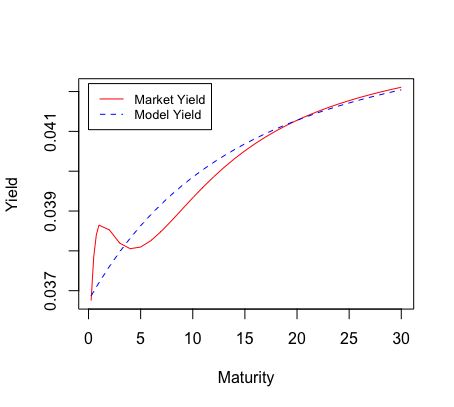
\includegraphics[scale = 0.7]{problem4_result.png}
		\caption{Market yield and model yield}
		\label{fig:prob4-result}
	\end{figure}
	Table \ref{tab:prob4-result} shows the optimization result.
	\begin{table}[!htbp]
\centering
\begin{tabular}{@{}cccccc@{}}
\toprule
Maturity(Year) & Yield(Market) & $G_0$    & $G_1$   & Yield(Model) & Absolute Error \\ \midrule
0.25     & 3.68\%        & -0.0001 & 0.2469 & 3.69\%       & 0.0001         \\
0.5      & 3.79\%        & -0.0006 & 0.4877 & 3.70\%       & 0.0009         \\
0.75     & 3.84\%        & -0.0013 & 0.7226 & 3.71\%       & 0.0013         \\
1        & 3.86\%        & -0.0022 & 0.9516 & 3.72\%       & 0.0014         \\
2        & 3.85\%        & -0.0086 & 1.8127 & 3.76\%       & 0.0009         \\
3        & 3.82\%        & -0.0187 & 2.5918 & 3.80\%       & 0.0002         \\
4        & 3.81\%        & -0.0321 & 3.2968 & 3.83\%       & 0.0003         \\
5        & 3.81\%        & -0.0485 & 3.9347 & 3.86\%       & 0.0005         \\
6        & 3.83\%        & -0.0677 & 4.5119 & 3.89\%       & 0.0007         \\
7        & 3.85\%        & -0.0892 & 5.0341 & 3.92\%       & 0.0007         \\
8        & 3.88\%        & -0.1130 & 5.5067 & 3.94\%       & 0.0007         \\
9        & 3.91\%        & -0.1387 & 5.9343 & 3.96\%       & 0.0006         \\
10       & 3.93\%        & -0.1662 & 6.3212 & 3.99\%       & 0.0005         \\
11       & 3.96\%        & -0.1953 & 6.6713 & 4.00\%       & 0.0004         \\
12       & 3.99\%        & -0.2258 & 6.9881 & 4.02\%       & 0.0004         \\
13       & 4.01\%        & -0.2577 & 7.2747 & 4.04\%       & 0.0003         \\
14       & 4.03\%        & -0.2907 & 7.5340 & 4.05\%       & 0.0002         \\
15       & 4.05\%        & -0.3248 & 7.7687 & 4.07\%       & 0.0002         \\
16       & 4.07\%        & -0.3598 & 7.9810 & 4.08\%       & 0.0001         \\
17       & 4.09\%        & -0.3957 & 8.1732 & 4.09\%       & 0.0001         \\
18       & 4.10\%        & -0.4324 & 8.3470 & 4.11\%       & 0.0001         \\
19       & 4.12\%        & -0.4698 & 8.5043 & 4.12\%       & 0.0000         \\
20       & 4.13\%        & -0.5078 & 8.6466 & 4.13\%       & 0.0000         \\
21       & 4.14\%        & -0.5464 & 8.7754 & 4.14\%       & 0.0000         \\
22       & 4.15\%        & -0.5855 & 8.8920 & 4.15\%       & 0.0000         \\
23       & 4.16\%        & -0.6251 & 8.9974 & 4.16\%       & 0.0000         \\
24       & 4.17\%        & -0.6651 & 9.0928 & 4.16\%       & 0.0001         \\
25       & 4.18\%        & -0.7055 & 9.1792 & 4.17\%       & 0.0001         \\
26       & 4.18\%        & -0.7463 & 9.2573 & 4.18\%       & 0.0001         \\
27       & 4.19\%        & -0.7873 & 9.3279 & 4.19\%       & 0.0001         \\
28       & 4.20\%        & -0.8287 & 9.3919 & 4.19\%       & 0.0001         \\
29       & 4.21\%        & -0.8702 & 9.4498 & 4.20\%       & 0.0001         \\
30       & 4.21\%        & -0.9121 & 9.5021 & 4.20\%       & 0.0001         \\ \bottomrule
\end{tabular}
\caption{Optimization Result: $r^* = 4.614\%$, average absolute error: 0.0003}
\label{tab:prob4-result}
\end{table}

\end{homeworkProblem}

%----------------------------------------------------------------------------------------
%	PROBLEM 5
%----------------------------------------------------------------------------------------

\begin{homeworkProblem}
	\begin{enumerate}[(a)]
		\item	%% problem (a)
		\item	%% problem (b)
		\item	%% problem (c)
	\end{enumerate}
\end{homeworkProblem}
\end{document}
